% phone type
% alignment

\section{實驗集與分析模型}
  
本研究的分析對象
參考
無文字架構 \cite{noauthor_textless_2021, lakhotia_generative_2021, lakhotia_generative_2021-1}  
研究,
採用當中
提及的 CPC、Wav2vec 2.0 和 HuBERT 三個語音基石模型,
並
與作為比對的
聲學特徵
梅爾時頻譜(Mel-Spectrogram),
一共四種語音表徵模型。
$$
\text{((寫一下 resolution 跟層數))}
$$
此後亦跟隨
該研究
選用
特定模型層數,
和其釋出的
K-平均量化模型。
%% ==========
這些模型層數與量化為該研究中
被證明與語音學特徵最相關,
且被使用於無文字架構後續研究之
語音離散表徵的抽取方法。
%% ==========
無文字研究中已透過
(某某)語料
對四種語音表徵
進行 K-平均分群演算法,
分別得到群數為 50、100 和 200 的三個量化模型。

%% ==========
本論文以公開的 LibriSpeech 資料集為分析對象,
採取其 train-clean-100 為分析的語音語料庫。
%% ==========
% 因此,
本研究將
語音語料庫的
語音資料
經過四個模型
獲取連續表徵後,
再經過量化模型
得到完全由離散單元組成的「偽文字」語料。

%% ==========
針對語音學的音位標註,
吾人透過 Montreal 強迫對齊器(Forced-Aligner) [[CITE montreal]]
的英語預訓練模型,
從語料庫的文字轉寫
取得
語音資料的音位標註
與對應的時間範圍。
最後透過
語音表徵各自的
時間解析度
生成
以音框為單位的
音位標註語料。
%% ==========
最後將兩者對語音資料集進行
音位標註
相關性的分析。



\section{分析結果}



%% \begin{center}
%% (((還是放一下長條圖說個事兒好了)))     
%% \end{center}
  
由表 \ref{tab:grouped_tables} 中可以看出,分群的群數愈多時,音位的純度確實有所上升,但這可能是犧牲分群純度得來的。因此再看 PNMI 的指標可以發現,整體離散單元和音位標註的相關性還是有所提升的。

此外,就不同模型來觀察,HuBERT 的表現是四種語音表徵之中最好的,一定程度上可以佐證 HuBERT 在找出語音中有意義單位上的效能,以及為什麼無文字架構通常以 HuBERT 當成抽取語音離散表徵的模型。

%%% \begin{center}
%%% 
%%% %% 「「「
%%% %% 終於要直面 code 了!
%%% %% 」」」
%%% \end{center}

% \begin{figure}
%     \centering
%     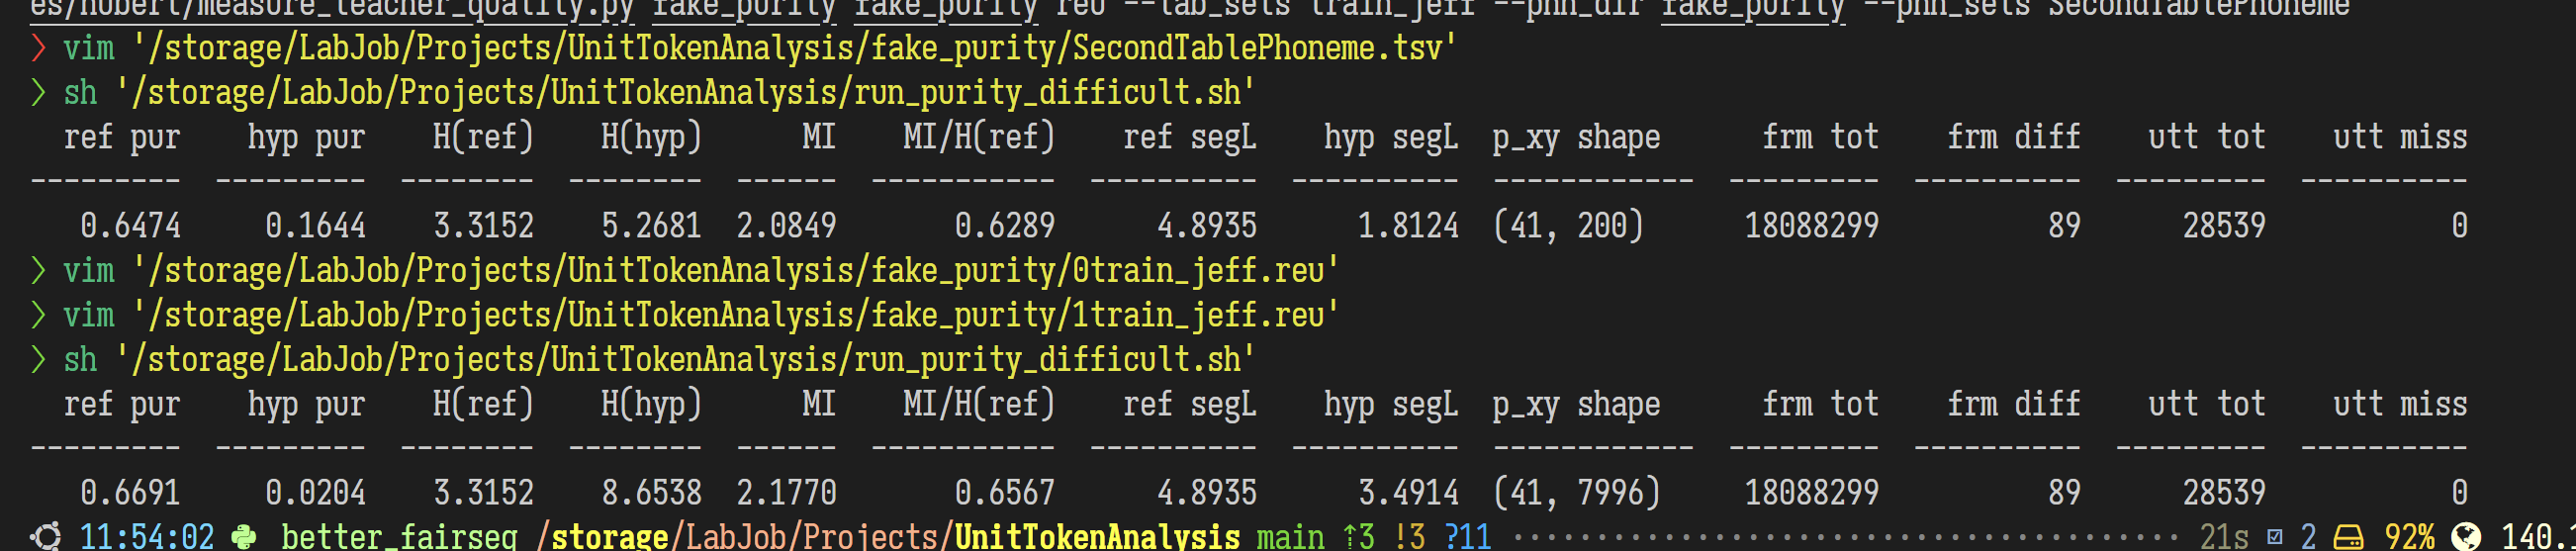
\includegraphics[width=0.75\linewidth]{figures/res1.png}
%     \caption{Enter Caption}
%     \label{fig:enter-label}
% \end{figure}








%% \documentclass{article}
%% \usepackage{caption}
%% \usepackage{subcaption}


\begin{table}[!htbp]
    \centering
    \begin{subtable}[t]{\textwidth}
        \centering
        \begin{tabular}{cccccc}
            %% 0 & refpur & hyppur & Href & Hhyp & MI\_pnmi\\
            & 音位純度 & 分群純度 & 音位熵 & 離散單元熵 & PNMI \\
            HuBERT      &   0.5256   &  0.3382 &   3.3152  &  3.8681    &     0.4993   \\   %% 1.6552 h
            wav2vec 2.0 &   0.4006   &  0.2676 &   3.3152  &  3.8215    &     0.3706   \\   %% 1.2286 w
            CPC         &   0.5188   &  0.3812 &   3.3146  &  3.7918    &     0.4992   \\   %% 1.6545 c
            LogMel      &   0.3253   &  0.1473 &   3.3158  &  3.8630    &     0.2647   \\   %% 0.8776 l
        \end{tabular}
        \caption{群數 = 50}
        \label{tab:ch3-clu050}
    \end{subtable}

    \vspace{0.5cm}

    \begin{subtable}[t]{\textwidth}
        \centering
        \begin{tabular}{cccccc}
            %% 0 & refpur & hyppur & Href & Hhyp & MI\_pnmi\\
            & 音位純度 & 分群純度 & 音位熵 & 離散單元熵 & PNMI \\
            HuBERT      &   0.6097   &  0.2553 &   3.3152  &  4.5704    &     0.5786   \\   %% 1.9181 h
            wav2vec 2.0 &   0.4877   &  0.2118 &   3.3152  &  4.5284    &     0.4596   \\   %% 1.5235 w
            CPC         &   0.5895   &  0.2674 &   3.3146  &  4.5034    &     0.5557   \\   %% 1.8418 c
            LogMel      &   0.3348   &  0.0931 &   3.3158  &  4.5591    &     0.2789   \\   %% 0.9247 l
        \end{tabular}
        \caption{群數 = 100}
        \label{tab:ch3-clu100}
    \end{subtable}

    \vspace{0.5cm}

    \begin{subtable}[t]{\textwidth}
        \centering
        \begin{tabular}{cccccc}
            %% 0 & refpur & hyppur & Href & Hhyp & MI\_pnmi\\
            & 音位純度 & 分群純度 & 音位熵 & 離散單元熵 & PNMI \\
            HuBERT      &   0.6474   &  0.1644 &   3.3152  &  5.2681    &     0.6289   \\   %% 2.0849 h
            wav2vec 2.0 &   0.5427   &  0.1467 &   3.3152  &  5.2173    &     0.5188   \\   %% 1.7199 w
            CPC         &   0.6098   &  0.1789 &   3.3146  &  5.1885    &     0.5882   \\   %% 1.9497 c
            LogMel      &   0.3474   &  0.0569 &   3.3158  &  5.2322    &     0.2955   \\   %% 0.9798 l
        \end{tabular}
        \caption{群數 = 200}
        \label{tab:ch3-clu200}
    \end{subtable}

    \caption{Grouped Tables}
    \label{tab:grouped_tables}
\end{table}





 

\section{本章總結}

  
本章節探討以音框為單位取出的語音離散表徵
與對應的音位標註之間的關係,
從分析結果中可以得到,
HuBERT 模型
的離散表徵
確實
與
人類
理解的
語音單位
「音位」
之間,
具有最明顯的相似性,
也進一步證明
% 以此尋找語音中的
為何
HuBERT 目前是
抽取語音離散表徵時最常使用的模型。
